\documentclass[a4paper,12pt]{article}
\usepackage[utf8]{inputenc}
\usepackage{wrapfig}
\usepackage{graphicx}
\usepackage{float}
\usepackage{amsmath}
\usepackage{pslatex}
\usepackage[portuguese]{babel}
\usepackage{indentfirst}
\usepackage{natbib}
\usepackage[textsize=tiny]{todonotes}
\usepackage{tikz}
\usepackage[lmargin=3cm,rmargin=3cm,tmargin=2.5cm,bmargin=2.5cm]{geometry}
\setlength{\parindent}{1cm}
\setlength{\baselineskip}{1.5cm}
\renewcommand{\contentsname}{Sumário}



\begin{document}

\begin{titlepage}
 \begin{center}
  { \large FUNDAÇÃO GETULIO VARGAS}\\[0.3cm]
  { \large ESCOLA DE MATEMÁTICA APLICADA}\\[0.5cm]
  { \large CURSO DE GRADUAÇÃO EM}\\[0.3cm]
  { \large MATEMÁTICA APLICADA}\\[0.3cm]
 
  \vspace{55 mm}

  {\bf \large Dinâmica de Disseminação de Notícias em}\\[0.1cm]
  {\bf \large Redes Complexas}\\[1.7cm]

  { por}\\[0.6cm]
  {\large Elisa Mussumeci}\\[0.1cm]


  \vspace{7cm}

  { Rio de Janeiro}\\[0.1cm]
  { 2015}\\[0.6cm]
  { FUNDAÇÃO GETÚLIO}\\[0.1cm]
  { VARGAS}\\[0.1cm]
 \end{center}
\end{titlepage}

\begin{titlepage}
 
 \begin{center}
  {\large FUNDAÇÃO GETULIO VARGAS}\\[0.3cm]
  {\large ESCOLA DE MATEMÁTICA APLICADA}\\[0.5cm]
  {\large CURSO DE GRADUAÇÃO EM}\\[0.3cm]
  {\large MATEMÁTICA APLICADA}\\[0.3cm]


  \vspace{20 mm}


  {\large Dinâmica de Disseminação de Notícias em}\\[0.1cm]
  {\large Redes Complexas}\\[2.5cm]

  
  \bf "Declaro ser o único autor do presente projeto de monografia que refere-se ao
plano de trabalho a ser executado para continuidade da monografia e ressalto
que não recorri a qualquer forma de colaboração ou auxílio de terceiros para
realizá-lo a não ser nos casos e para os fins autorizados pelo professor orientador"

  \vspace{3.5cm}


  \line(1,0){220}\\[0.1cm]
  {\bf Elisa Mussumeci}\\[2cm]
  {\bf Orientador: Flavio Codeço Coelho}\\[5cm]




  {Rio de Janeiro}\\[0.1cm]
  {2015}
 \end{center}
\end{titlepage}

\begin{titlepage}
 \begin{center}
 
  {\bf \large ELISA MUSSUMECI}\\[0.3cm]

  \vspace{25 mm}

  {\bf \large Dinâmica de Disseminação de Notícias em}\\[0.1cm]
  {\bf \large Redes Complexas}\\[4cm]

  {“Monografia apresentada à Escola de Matemática Aplicada}\\[0.1cm]
  {como requisito parcial para obtenção do grau de Bacharel }\\[0.1cm]
  {em Matemática Aplicada”}\\[6cm]


  {Aprovado em \ \line(1,0){20} \ \ de \line(1,0){62} \ \ de \line(1,0){30} \ .}\\[0.1cm]
  {Grau atribuido ao Projeto de Monografia: \line(1,0){20} \ . }\\[3cm]
  
  
  {\line(1,0){250}}\\
  {\bf Professor Orientador: Flávio Codeço Coelho}\\[0.1cm]
  {\bf Escola de Matemática Aplicada}\\[0.1cm]
  {\bf Fundação Getulio Vargas}
 \end{center}
\end{titlepage}

\newpage\null\thispagestyle{empty}\newpage

\tableofcontents

\pagebreak

\begin{abstract}
 
O processo de formação de opinião é fortemente influenciado pela mídia digital.
Entretanto pouco se sabe sobre o processo de disseminação de notícias e os fatores que determinam o alcance de cada
notícia.

A disseminação de uma notícia se dá por meio de um ou mais caminhos em uma rede desconhecida de influência entre 
formadores de opinião (produtores de notícias). Este padrão pode ser recuperado, com algum grau de incerteza, a partir de dados
da sequência temporal das publicações sobre um mesmo tema, e dos links nelas contidos.

Este projeto tem como objetivo caracterizar as redes de interligação de veículos de mídia e modelar a dinâmica do espalhamento 
de notícias, a fim de prever tendências e mapear questões de interesse.

\end{abstract}

\pagebreak

\section{Introdução}


Atualmente a internet é um dos principais meios de veiculação de notícias e informação do país. Com o crescente
número de pessoas aderindo à redes sociais, o compartilhamento de notícias aumentou significamente, o que tornou fundamental
o papel das mídias digitais no acesso à informação.

Consideramos como mídia digital todo e qualquer veículo difusor de informação contido na internet brasileira, como jornais, revistas e 
blogs independentes. Cada mídia presente na internet possui sua própria periodicidade, alcance, público e credibilidade, o que afeta
diretamento no processo de disseminação da informação.

Utilizando do fato que essas mídias digitais são fundamentais na disseminação da informação, e que com isso possuem um forte papel 
influenciador no processo de formação de opinião, podemos definir como importante entender como as notícias se formam e se espalham
na internet brasileira.

Um dos métodos de se estudar a disseminação da informação é utilizar modelos epidemiológicos. (referencia de artigo) em (ano do artigo)
conseguiu modelar a disseminação de (tabela de alguma coisa) no tempo através de modelos epidemiológicos, como SIR, SIS entre outros. Ese tipo
de abordagem vem sendo utilizada também para entender redes de contatos em redes sociais como (incluir referencia). MELHORAR PARAGRAFO

Neste trabalho utilizaremos redes complexas e modelos epidemiológicos para modelar a disseminação de notícias na mídia brasileira. 
Para isso
estudaremos os caminhos percorridos em uma rede de disseminação criada através de modelos de recuperação de informação utilizados em cima
da base de dados do Projeto MediaCloud Brasil \todo{referência}.

\subsection{O Projeto Media Cloud Brasil}

Para a realização deste trabalho, foram utilizados os dados do projeto MediaCloud Brasil. O MediaCloud Brasil é um projeto concebido e mantido pelo
NAMD/EMAp da Fundação Getúlio Vargas, e vem ao longo dos últimos três anos monitorando mais de cem mil veículos de mídia da internet brasileira. Possui em
sua base de dados mais de 1.6 milhão de artigos capturados.
\todo[inline]{falar sobre o que e como o Media cloud captura os artigos}
O projeto utiliza como banco de dados o MongoDB, um banco de dados de documentos open-source de alta performance. O MongoDB é classificado como um banco de 
dados 'NoSQL', uma vez que evita a tradicional estrutura  baseada em tabela relacional e utiliza documentos JSON com esquemas dinâmicos para armazenamento 
dos documentos. A vantagem de utilizar o JSON é realizar a integração de dados em certos tipos de aplicações de forma mais fácil e mais rápida.\todo{Que tipo de aplicações?}
\todo[inline]{Falar que uma vez armazenado, o banco de artigos é indexado para permitir buscas textuais}

\subsection{Referencial Teórico}


\subsubsection{O espalhamento de notícias como um processo de contágio}

Uma epidemia é caracterizada pela incidência de grande número de casos de uma doença em um curto período de tempo. Sabemos que as doenças
se espalham através do contágio entre infectados, mas como podemos definir esse contágio? 

Cada doença possui uma forma própria de transmissão, por exemplo, a gripe é uma doença viral e se transmite a partir de vias orais, já a dengue
é transmitida a partir da picada de um mosquisto, assim como a febre amarela. Saber a forma de contágio de uma doença é fundamental para que
possamos entender sua disseminação e modelar sua epidemia.

Ao observar o comportamento de notícias, assuntos e histórias na mídia, podemos ver o surgimento de memes e histórias 'virais'. Esses 
tipos de notícias são chamadas de virais por se espalharem muito rápido e obterem um alcançe grande na população. Algumas dessas notícias
se sustentam por um longo tempo na mídia, e outras são esquecidas rapidamente. 

Se pensarmos que estamos lidando com um processo de disseminação, que possui uma taxa de espalhamento e uma taxa de esquecimento, podemos
facilmente fazer uma comparação à modelos epidemiológicos, principalmente ao modelo SIR, que possui uma taxa de infecção e
uma taxa de recuperação. Dessa forma, podemos estudar como uma notícia se espalha da mesma forma que modelamos uma epidemia.

Para modelar a disseminação de notícias da mesma forma que modelamos a de doenças, precisamos
que nosso modelo seja compatível com o de uma epidemia, ou seja, precisamos definir os infectados, suscetíveis e o método de contágio.

Em nosso modelo, uma notícia/assunto é a doença, e os infectados são todos os artigos que falam sobre essa notícia. 
Para definir o contágio da nossa notícia, consideramos que um artigo infecta o outro quando ele influência o outro. Ou seja,
definimos que quando um artigo exerceu influência sobre um outro, ele infectou esse outro artigo. 

Dessa forma, podemos ver a similaridade entre ambas modelagens, o que deixa claro a possibilidade de modelar a disseminação de
notícias através de modelos epidemiológicos. O que nos falta descobrir são os parâmetros que utilizaremos para realizar essa modelagem
de forma que fique o mais verídica possível.

\subsubsection{Processos Epidemiológicos em Redes Complexas}

O termo Redes Complexas se refere a um grafo que apresenta uma estrutura topográfica não trivial, composto por um conjunto
 de vértices (nós) que são interligados por meio de arestas (Barabási, 2003). A teoria das Redes Complexas  está relacionada com a modelagem de redes reais, através da 
 análise de dados empíricos. Redes Complexas não são estáticas (evoluem no tempo alterando sua estrutura), e 
 constituem estruturas onde processos dinâmicos (como disseminação de virus ou opiniões) podem ser simulados.
 
 
\subsubsection{Processamento de Linguagem Natural}
\label{sec:nlp}

\todo[inline]{explicar aqui a teoria por trás de todas as técnicas de NLP que vc usa: Tokenização, TF-IDF, etc.}
representação vetorial de palavras

\begin{description}
 \item \textbf{Tokenização}
 \item \textbf{TF-IDF}
 
O modelo Tf-Idf (\textit{term frequency-inverse document frequency}), é uma medida estatística que tem o intuito de indicar
a importância de uma palavra de um documento em relação a um corpus linguístico muito usada para rankeamento de documentos em uma consulta. O Tf-Idf trata-se do produto entre as estatísticas $Tf_{d,t}$ e
$Idf_{t}$.


Dado um conjunto de $N$ documentos, $Tf_{d,t}$ é a frequência do termo $t$ no documento
$d$, ou seja, o número de vezes em que $t$ ocorre em $d$. Usamos o termo $Tf$ para computar escores de correspondência consulta-documento,
porém, o $Tf$ nos dá a frequência absoluta dos termos, o que faz com que um termo que possua $Tf=10$ seja 10 vezes mais relevante do um que possua
$Tf=1$. 

Podemos concordar que um documento com $Tf=10$ é mais relevante do que um com $Tf=1$, porém não necessariamente 10 vezes mais relevante.
A relevância não aumenta em proporção com a frequência do termo. Para contornar isso, é comum usar ao invés da frequência absoluta uma ponderação
pelo $Log$ da frequência. Dessa forma, o peso $log$ da frequência do termo $t$ em $d$ é definido como:

\begin{equation}
  W_{t,d}=\begin{cases}
	    1 + logTf_{t,d}  \hspace{1cm} \text{se} \ Tf_{t,d} > 0 \\
	    0 \ \hspace{3cm} \text{caso contrário}
	  \end{cases}
\end{equation}


Exemplificamos abaixo a correspondência de valores $Tf_{t,d}$ absoluto com a ponderação $W_{t,d}$:

\begin{center}
\begin{tabular}{ll}
  \hline
  $Tf_{t,d}$ & $W_{t,d}$\\
  \hline
  0&0\\
  1&1\\
  2&1.3\\
  10&2\\
  1000&4\\
  
\end{tabular}
\end{center}


Sabemos que nem todo termo frequente em um documento pode ser considerado muito relevante. Consideramos uma consulta com dois termos:
um frequente no conjunto de documentos e outro raro. Não queremos que um documento que possua o termo frequente seja mais relevante do que o
documento que possua o termo raro.

Inferimos então que termos raros são mais informativos do que termos frequentes. Dessa forma, queremos dar uma maior relevância para
termos raros do que para termos muito frequentes. Para incluir isso em nossa medida usamos o termo $Idf$.

O termo $Idf_{t}$ é uma medida de informatividade do termo $t$, que afeta o rankeamento de documentos para consultas com pelo menos dois
termos. Com ele aumentamos o peso relativo de termos raros e diminuimos o peso relativo
de termos muito frequentes. O definimos da seguinte maneira:

$$ Idf_{t}\ = \ log\ \frac{N}{df_{t}}$$

Onde $df_{t}$ é a frequência de documento, o número de documentos em que $t$ ocorre. Consideramos $df_{t}$ uma medida inversa da informatividade
do termo $t$.

Ao multiplicarmos o termo $Idf$ ao nosso peso ponderado $W_{t,d}$, temos a medida Tf-Idf. O peso Tf-Idf aumenta com o número de ocorrências
dentro de um documento e com a raridade do termo na coleção. É considerado o melhor esquema de ponderação em recuperação da informação.

$$ W_{t,d} = (1 + log Tf_{t,d}) \cdot \ log \dfrac{N}{Df_{t}}$$

\item \textbf{Bag-of-Words}
\item \textbf{Skipgram}

Explicar pq é um modelo adequado para o meu problema
\end{description}

\section{Objetivo}

Esse trabalho tem como principal objetivo caracterizar a dinâmica de disseminação das notícias no país através de redes complexas.




\pagebreak
\section{Metodologia}

\subsection{Rede de Disseminação Real}

Nesta primeira parte do trabalho, iremos construir uma rede complexa que descreva o processo epidemiológico de uma notícia. O objetivo
da construção dessa rede, é conseguir aproximar a rede de interligação real entre os artigos selecionados do banco
MediaCloud, de forma a torná-la observável.

Primeiramente, selecionamos todos os artigos do banco referentes a uma determinada notícia, criando assim, nosso corpus linguístico.
Depois ,a partir desse corpus, utlizamos métodos de PLN para representar matricialmente nosso conjunto de dados. A partir da matriz 
criada construímos nossa rede direcionada de disseminação, onde cada vértice ou nó da rede é um artigo.

Para construir a rede de disseminação precisamos definir a relação de contágio entre artigos, ou seja, o que conecta um artigo ao outro 
na rede. No nosso caso, definimos que o contágio se dá através de uma relação de influência, porém como definir essa relação? Partindo do
pressuposto de que se um artigo influênciou outro então esses artigos são necessariamente similares, consideramos a \textbf{similaridade}
entre os artigos o fator principal para definir se eles possuem uma conexão em nossa rede.

Possuindo uma conexão, ainda precisamos saber quem influênciou e quem foi o influenciado. Para definir isso, utilizamos o \textbf{tempo}.
Assim, dado que dois artigos são similares, definimos como influenciador o artigo que fui publicado primeiro e influenciado o artigo publicado
depois. No caso de um artigo ter mais de um similar publicado anteriormente a ele, definimos como influenciador o artigo
mais similar à ele. Dessa forma todos os vértices de nossa rede possuem um grau de entrada igual à 1 e podem possuir um grau de saída maior
do que 1.

A seguir, podemos ver um exemplo do que esperamos da nossa rede de disseminação real:


\begin{figure}[h]
 \centering
 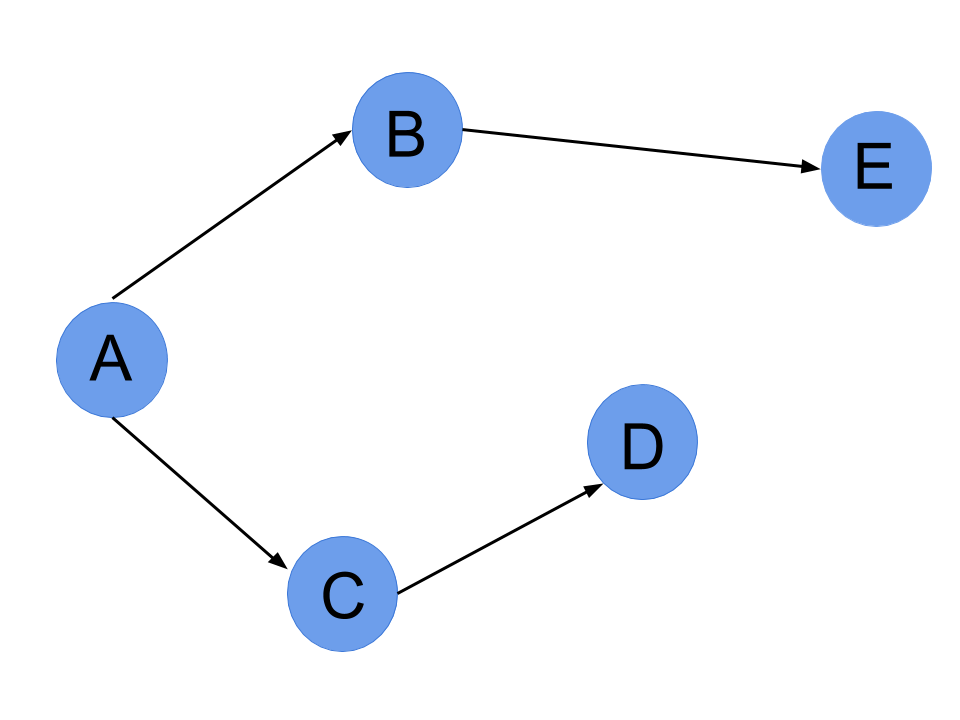
\includegraphics[scale=0.2]{./rede1.png}
 % rede1.png: 960x720 pixel, 72dpi, 33.87x25.40 cm, bb=0 0 960 720
 \caption{Rede Real Genérica}
\end{figure}

No exemplo acima, temos que o artigo $A$ é similar aos artigos $B$ e $C$ e possui uma data de publicação mais antiga do que os dois. 
Sendo assim, foi definido como o influenciador dos dois, ou seja, foi o artigo que os contagiou com a notícia.

\subsubsection{Matriz de Documentos}

Selecionamos no banco de dados do MediaCloud todos os artigos referentes a uma determinada notícia, formando o corpus linguístico que 
utilizaremos para criar a matriz de documentos, representação vetorial dos artigos selecionados.

Para representar vetorialmente nosso conjunto de dados utilizamos o \textit{Word2Vec}, ferramenta que promove uma implementação 
eficiente do modelo \textit{skip-gram} e \textit{bag-of-words} contínuo (inserir referencia).\todo{preciso explicar mais sobre o word2vec?}

Para gerar nosso modelo Word2Vec \todo{preciso explicar que tem que haver um conjunt trainado com todos os artigos do mediacloud etcs?}, fornecemos como entrada nosso corpus linguístico
e o modelo nos retorna uma matriz, onde as linhas $p_{1},p_{2},...,p_{n}$ são as palavras contidas no corpus e as colunas $t_{1},t_{2},...,t_{n}$
são os atributos gerados pelo modelo para cada palavra:
 
 \begin{center}
 \hspace{0.2cm}$t_{1}$ \hspace{0.5cm} $t_{2}$ \hspace{0.3cm} $\hdots$ \hspace{0.4cm}$t_{n}$
 
 \vspace{0.2cm}
 
\begin{tabular}{c}
   $p_{1}$ \\
   $p_{2}$ \\
   \vdots\\
   $p_{n}$
 \end{tabular}
 $
 \begin{bmatrix}
  a_{11} & a_{12} & \hdots & a_{1n}\\
  a_{21} & a_{22} & \hdots & a_{2n}\\
  \vdots & \vdots & \ddots & \vdots\\
  a_{31} & a_{32} & \hdots & a_{nn}
 \end{bmatrix}_{nxn}
$

\end{center}

Dessa forma, temos uma matriz de palavras, ou seja, uma representação de todas as palavras presentes em nosso corpus.
Porém, queremos representar documentos e não apenas palavras.
Para criar uma matriz que represente documentos, fazemos, para cada documento, uma soma dos vetores referentes a cada palavra presente
no documento, criando assim um vetor representativo do documento em questão.

Podemos exemplificar da seguinte forma: dado um documento $D$, sabemos que ele é composto pelo seguinte conjunto de palavras
$P:\{1,2,3,4,5\}$. Para cada termo, buscamos o seu vetor representativo $p_{i}$, $i =\{1,2,3,4,5\}$ na matriz de
palavras e somamo-os, criando o vetor $v_{D}$ que representa o vetor referente ao documento $D$:

$$v_{D} = p_{1}+p_{2}+p_{3}+p_{4}+p_{5} $$

Ao representar um documento dessa forma, não levamos em consideração a relevância de cada palavra para o documento, o que
faz da nossa representação pouco eficiente. Para melhorar nossa 
eficiência, antes de somar os vetores de palavras $p_{i}$, iremos multiplicar cada um deles pelo valor \textit{TF-IDF} da palavra
ao qual ele representa.

Sendo assim, sabendo que para cada palavra $i$ temos um vetor $p_{i}$ que a representa na matriz de palavras, e um valor $w_{i,d}$ referente
ao valor \textit{TF-IDF} da palavra $i$ no documento $D$, representamos o vetor $v_{D}$ da seguinte forma:

  $$v_{D} = \sum_{i=1}^{5} p_{i} \cdot w_{t,D} $$

Sendo assim, ficamos com a matriz de documentos abaixo, onde cada linha $v_{i}$ é um documento, e cada coluna $t_{i}$ é a soma do atributo $i$
em todas as palavras do documento $i$:

 \begin{center}
 \hspace{0.2cm}$t_{1}$ \hspace{0.5cm} $t_{2}$ \hspace{0.3cm} $\hdots$ \hspace{0.4cm}$t_{n}$
 
 \vspace{0.2cm}
 
\begin{tabular}{c}
   $v_{1}$ \\
   $v_{2}$ \\
   \vdots\\
   $v_{n}$
 \end{tabular}
 $
 \begin{bmatrix}
  a_{11} & a_{12} & \hdots & a_{1n}\\
  a_{21} & a_{22} & \hdots & a_{2n}\\
  \vdots & \vdots & \ddots & \vdots\\
  a_{31} & a_{32} & \hdots & a_{nn}
 \end{bmatrix}_{nxn}
$

\end{center}



\subsubsection{Construção da Rede}

 Construimos a rede de disseminação a partir da matriz de documentos gerada na sessão anterior, onde cada vetor consiste em um documento/artigo.
 
 Ao construir a rede dos nossos documentos,
 consideramos como contágio sofrer influência de outro artigo, ou seja, um artigo A contamina um artigo B se o artigo A influenciou o
 artigo B.
 
 Dessa forma, em nossa rede, os vértices representam os artigos, e as arestas a relação de influência entre eles, isto é, dado um nó $e_{i}$ e um nó
 $e_{j}$, existe uma aresta $a_{ij}$, que sai de \textit{i} e vai para \textit{j}, se o artigo \textit{i} influênciou o artigo \textit{j}.
 
 Para definir quando um artigo influência outro em nossa rede, foram usadas duas heurísticas: \textit{similaridade} e 
 \textit{temporalidade}.
 
 \begin{description}
  \item \textbf{Similaridade}
  
    Para definir similaride entre dois artigos, utilizamos a \textit{Similaridade de Cosseno}. A similaridade de cosseno mede a semelhança entre
    dois vetores através da distância de cosseno do ângulo que eles formam. Para calcular a distância de cosseno $d(A,B)$ entre um vetor $A$ e $B$, fazemos:
    
    $$ d(A,B) = cos(\theta) = \dfrac{A \cdot B}{\parallel A\parallel \parallel B \parallel} $$
    
    A similaridade de cosseno se dá por $1-d(A,B)$.Utilizando essa equação, calculamos a similaridade de cosseno para cada
    par de vetor de nossa matriz de documentos, criando assim, uma matriz de similaridades. Se similaridade entre dois vetores for 
    grande o suficiente, os definimos como similares. 
    
    Para saber o quão grande a similaridade de cosseno entre dois artigos deve ser para considerarmo-os similares, fazemos a
    distribução das similaridade e realizamos um corte em suas extremidades.
    
    
  \item \textbf{Temporalidade}
  
    Após definir dois artigos como similares, inferimos uma relação de influência entre eles. Porém, ainda precisamos saber quem influeciou e quem
    foi influenciado. Para descobrir isso, olhamos a data de publicação de cada artigo. Se dois artigos $A$ e $B$ foram considerados 
    similares, e o artigo $A$ foi publicado antes do artigo $B$, então definimos que $A$ influenciou $B$, logo temos em nossa rede:
    
    \begin{figure}[h]
      \centering
      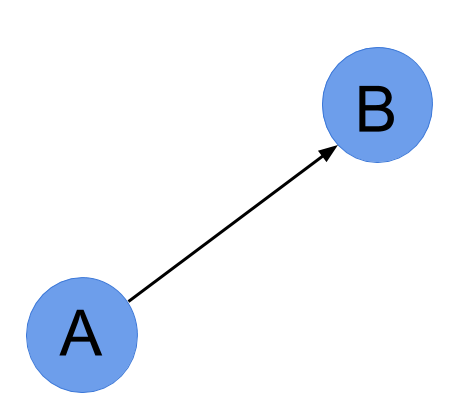
\includegraphics[scale=0.2]{./rede2.png}
      % rede2.png: 960x720 pixel, 72dpi, 33.87x25.40 cm, bb=0 0 960 720
      \caption{Relação de Influência}
    \end{figure}

    Porém, pode acontecer de termos um outro artigo $C$, também considerado similar ao artigo $B$ e que também publicado anteriormente. Em nosso modelo,
    definimos que um artigo só pode ter sido influênciado por um único artigo. Dessa forma, como definir quem de fato influênciou $B$? Para
    resolver esse impasse utilizamos a similaridade de cosseno. Consideramos influênciador o artigo publicado anteriormente, e que possui
    a \textbf{maior} similaridade com $B$.
    
    
 \end{description}
 

\subsection{Simulação Rede de Disseminação}

Nesta parte do trabalho, temos como objetivo simular a disseminação de nossa rede original utilizando o modelo (adicionar referencia)
para tentar validar nossa rede de disseminação como um processo epidemiológico.

\subsubsection{Rede Completa}

 Para simular nossa rede, construimos primeiramente uma rede completa com os mesmos nós de nossa rede original, onde os pesos das arestas
 são as probabilidades dessa aresta existir no caminho de disseminação da notícia, ou seja, a probabilidade de um artigo influenciar um 
 outro. Para isso, levamos em conta o veículo que publicou o artigo. Dessa forma podemos saber 
 através dos veículos qual a chance de um artigo do veículo x ser influenciado por um artigo do veículo y.

 Construimos então, uma matriz de pesos identificando todos os veículos presentes na rede original e contando quantas vezes
 cada veículo x foi influenciado pelo veículo y. Dado que na rede original possuimos n
 veículos diferentes, temos uma matriz quadrada $nxn$, onde cada posição $a_{ij}$ nos da a quantidade de vezes que o veículo i foi influenciado
 pelo veículo j. Consideramos que um veículo não influência a si mesmo, logo a diagonal da nossa matriz é de zeros:
 \pagebreak
 
 \begin{center}
 \hspace{0.2cm}a \hspace{0.5cm} b \hspace{0.3cm} $\hdots$ \hspace{0.4cm}c
 
 \vspace{0.2cm}
 $
 \begin{tabular}{c}
   a \\
   b \\
   \vdots\\
   c
 \end{tabular}
$
 $
 \begin{bmatrix}
  0 & a_{12} & \hdots & a_{1n}\\
  a_{21} & 0 & \hdots & a_{2n}\\
  \vdots & \vdots & \ddots & \vdots\\
  a_{31} & a_{32} & \hdots & 0
 \end{bmatrix}_{nxn}
$

\end{center}

\vspace{0.4cm}
Por exemplo, $a_{12}$ é o número de vezes que artigos do veículo $b$ influenciaram artigos do veículo $a$.

A partir da matriz de pesos damos os pesos de cada aresta de nossa rede completa. Para cada nó da rede, identificamos seu veículo e atribuimos
a todas as arestas que saem dele as chances dele influenciar cada vizinho, e a todas as arestas que chegam nele as chances dele ser influenciado
por cada vizinho:

[DESENHO REDE COMPLETA GENERICA]

\subsubsection{Simulação}

 Na simulação da disseminação, utilizamos o modelo epidemiológico [incluir referencia]:

 \begin{equation}
  \begin{cases}

   \dfrac{d\rho^{I}_{i}}{dt} = -\rho^{I}_{i}(t) + \lambda\rho_{i}^{S}(t) \sum_{j=1}^{N} a_{ij}\rho_{j}^{I}(t) \\     
   \dfrac{d\rho^{S}_{i}}{dt} = - \lambda\rho_{i}^{S}(t) \sum_{j=1}^{N} a_{ij}\rho_{j}^{I}(t)
   
  \end{cases}
 \end{equation}


   [EXPLICAR MODELO]
  
  Ao terminar a simulação obtemos uma matriz de estados, onde cada posição $a_{ij}$ se refere a probabilidade do artigo
  j estar contaminado no passo i da simulação. Utilizando uma distribuição de bernoulli, definimos os artigos que estão infectados
  em casa passo, ficando assim com uma matriz booleana de estados.
  
  A partir da matriz booleana, podemos criar todos os nós de nossa rede simulada. Porém, ainda precisamos criar as arestas, ou seja, definir
  as relações de influência. 
  
  Para definir as relações de influência, a cada novo artigo contaminado no passo $i$, consideramos como possíveis influenciadores todos os artigos
  infectados no passo $i-1$. Utilizando a matriz de pesos entre os domínios, calculamos a probabilidade de cada artigo infectado no tempo
  $i-1$ ter infectado cada novo artigo infectado no tempo $i$. Definimos o artigo influenciador a partir da probabilidade que ele tem de 
  influenciar o novo artigo infectado. 

  
  
\section{Resultados}
 


\subsection{Rede de Disseminação Original}

Abaixo temos uma visualização da
 rede criada:

\begin{figure}[h]
 \centering
 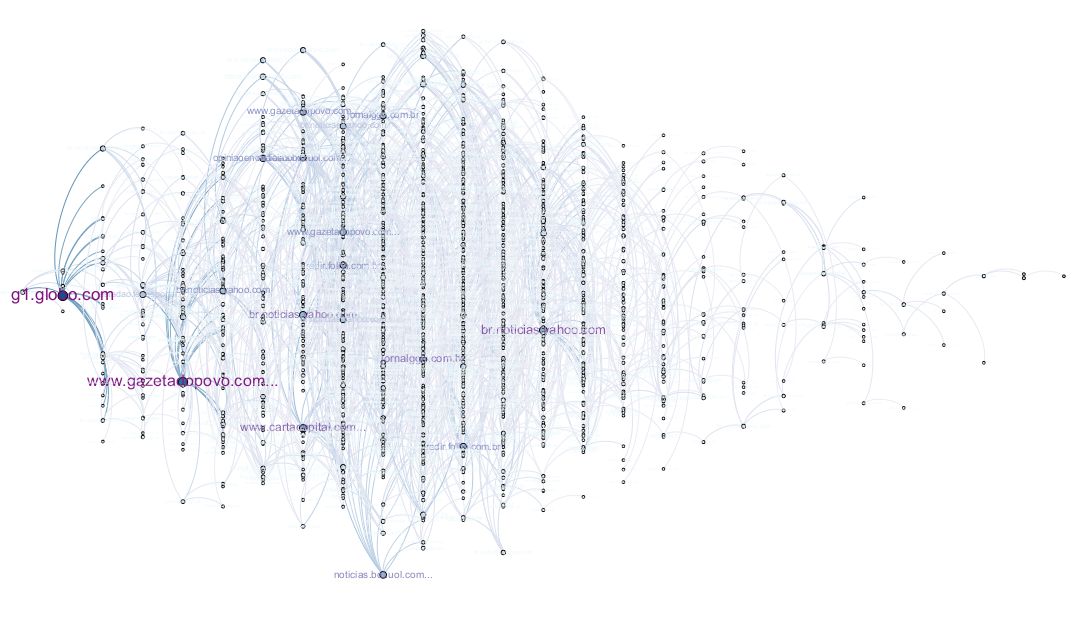
\includegraphics[scale=0.4]{../results/a.png}
 % a.png: 1075x623 pixel, 72dpi, 37.92x21.98 cm, bb=0 0 1075 623
 \caption{Rede Disseminação}
\end{figure}



\subsection{Simulação Rede de Disseminação}


\section{Conclusão}

\end{document}
